\documentclass[10pt,ignorenonframetext,,aspectratio=149]{beamer}
\usefonttheme{serif} % use mainfont rather than sansfont for slide text
\setbeamertemplate{caption}[numbered]
\setbeamertemplate{caption label separator}{: }
\setbeamercolor{caption name}{fg=normal text.fg}
\usepackage{lmodern}
\usepackage{amssymb,amsmath}
\usepackage{ifxetex,ifluatex}
\usepackage{fixltx2e} % provides \textsubscript
\ifnum 0\ifxetex 1\fi\ifluatex 1\fi=0 % if pdftex
  \usepackage[T1]{fontenc}
  \usepackage[utf8]{inputenc}
\else % if luatex or xelatex
  \ifxetex
    \usepackage{mathspec}
  \else
    \usepackage{fontspec}
  \fi
  \defaultfontfeatures{Ligatures=TeX,Scale=MatchLowercase}
  \newcommand{\euro}{€}
    \setmainfont[]{Open Sans}
\fi
% use upquote if available, for straight quotes in verbatim environments
\IfFileExists{upquote.sty}{\usepackage{upquote}}{}
% use microtype if available
\IfFileExists{microtype.sty}{%
\usepackage{microtype}
\UseMicrotypeSet[protrusion]{basicmath} % disable protrusion for tt fonts
}{}
\usepackage{graphicx,grffile}
\makeatletter
\def\maxwidth{\ifdim\Gin@nat@width>\linewidth\linewidth\else\Gin@nat@width\fi}
\def\maxheight{\ifdim\Gin@nat@height>\textheight0.8\textheight\else\Gin@nat@height\fi}
\makeatother
% Scale images if necessary, so that they will not overflow the page
% margins by default, and it is still possible to overwrite the defaults
% using explicit options in \includegraphics[width, height, ...]{}
\setkeys{Gin}{width=\maxwidth,height=\maxheight,keepaspectratio}

% Comment these out if you don't want a slide with just the
% part/section/subsection/subsubsection title:
\AtBeginPart{
  \let\insertpartnumber\relax
  \let\partname\relax
  \frame{\partpage}
}
\AtBeginSection{
  \let\insertsectionnumber\relax
  \let\sectionname\relax
  \frame{\sectionpage}
}
\AtBeginSubsection{
  \let\insertsubsectionnumber\relax
  \let\subsectionname\relax
  \frame{\subsectionpage}
}

\setlength{\emergencystretch}{3em}  % prevent overfull lines
\providecommand{\tightlist}{%
  \setlength{\itemsep}{0pt}\setlength{\parskip}{0pt}}
\setcounter{secnumdepth}{0}

\title{Analisis Digital}
\subtitle{(Sebuah metode dan Pendekatan)}
\author{Ujang Fahmi}
\date{}

%% Here's everything I added.
%%--------------------------

\usepackage{graphicx}
\usepackage{rotating}
%\setbeamertemplate{caption}[numbered]
\usepackage{hyperref}
\usepackage{caption}
\usepackage[normalem]{ulem}
%\mode<presentation>
\usepackage{wasysym}
%\usepackage{amsmath}


% Get rid of navigation symbols.
%-------------------------------
\setbeamertemplate{navigation symbols}{}

% Optional institute tags and titlegraphic.
% Do feel free to change the titlegraphic if you don't want it as a Markdown field.
%----------------------------------------------------------------------------------
\institute{Kedata Indonesia Digital}

% \titlegraphic{\includegraphics[width=0.3\paperwidth]{\string~/Dropbox/teaching/clemson-academic.png}} % <-- if you want to know what this looks like without it as a Markdown field. 
% -----------------------------------------------------------------------------------------------------
\titlegraphic{
\includegraphics[width=0.3\paperwidth]{images/kedata.png}}

% Some additional title page adjustments.
%----------------------------------------
\setbeamertemplate{title page}[empty]
%\date{}
\setbeamerfont{subtitle}{size=\small}

\setbeamercovered{transparent}

% Some optional colors. Change or add as you see fit.
%---------------------------------------------------
\definecolor{clemsonpurple}{HTML}{522D80}
 \definecolor{clemsonorange}{HTML}{F66733}
\definecolor{uiucblue}{HTML}{003C7D}
\definecolor{uiucorange}{HTML}{F47F24}


% Some optional color adjustments to Beamer. Change as you see fit.
%------------------------------------------------------------------
\setbeamercolor{frametitle}{fg=clemsonpurple,bg=white}
\setbeamercolor{title}{fg=clemsonpurple,bg=white}
\setbeamercolor{local structure}{fg=clemsonpurple}
\setbeamercolor{section in toc}{fg=clemsonpurple,bg=white}
% \setbeamercolor{subsection in toc}{fg=clemsonorange,bg=white}
\setbeamercolor{footline}{fg=clemsonpurple!50, bg=white}
\setbeamercolor{block title}{fg=clemsonorange,bg=white}


\let\Tiny=\tiny


% Sections and subsections should not get their own damn slide.
%--------------------------------------------------------------
\AtBeginPart{}
\AtBeginSection{}
\AtBeginSubsection{}
\AtBeginSubsubsection{}

% Suppress some of Markdown's weird default vertical spacing.
%------------------------------------------------------------
\setlength{\emergencystretch}{0em}  % prevent overfull lines
\setlength{\parskip}{0pt}


% Allow for those simple two-tone footlines I like. 
% Edit the colors as you see fit.
%--------------------------------------------------
\defbeamertemplate*{footline}{my footline}{%
    \ifnum\insertpagenumber=1
    \hbox{%
        \begin{beamercolorbox}[wd=\paperwidth,ht=.8ex,dp=1ex,center]{}%
      % empty environment to raise height
        \end{beamercolorbox}%
    }%
    \vskip0pt%
    \else%
        \Tiny{%
            \hfill%
		\vspace*{1pt}%
            \insertframenumber/\inserttotalframenumber \hspace*{0.1cm}%
            \newline%
            \color{clemsonpurple}{\rule{\paperwidth}{0.4mm}}\newline%
            \color{clemsonorange}{\rule{\paperwidth}{.4mm}}%
        }%
    \fi%
}

% Various cosmetic things, though I must confess I forget what exactly these do and why I included them.
%-------------------------------------------------------------------------------------------------------
\setbeamercolor{structure}{fg=blue}
\setbeamercolor{local structure}{parent=structure}
\setbeamercolor{item projected}{parent=item,use=item,fg=clemsonpurple,bg=white}
\setbeamercolor{enumerate item}{parent=item}

% Adjust some item elements. More cosmetic things.
%-------------------------------------------------
\setbeamertemplate{itemize item}{\color{clemsonpurple}$\bullet$}
\setbeamertemplate{itemize subitem}{\color{clemsonpurple}\scriptsize{$\bullet$}}
\setbeamertemplate{itemize/enumerate body end}{\vspace{.6\baselineskip}} % So I'm less inclined to use \medskip and \bigskip in Markdown.

% Automatically center images
% ---------------------------
% Note: this is for ![](image.png) images
% Use "fig.align = "center" for R chunks

\usepackage{etoolbox}

\AtBeginDocument{%
  \letcs\oig{@orig\string\includegraphics}%
  \renewcommand<>\includegraphics[2][]{%
    \only#3{%
      {\centering\oig[{#1}]{#2}\par}%
    }%
  }%
}

% I think I've moved to xelatex now. Here's some stuff for that.
% --------------------------------------------------------------
% I could customize/generalize this more but the truth is it works for my circumstances.

\ifxetex
\setbeamerfont{title}{family=\fontspec{Titillium Web}}
\setbeamerfont{frametitle}{family=\fontspec{Titillium Web}}
\usepackage[font=small,skip=0pt]{caption}
 \else
 \fi

% Okay, and begin the actual document...

\begin{document}
\frame{\titlepage}

\begin{frame}[fragile]
dSalam kenal, saya adalah Ujang Fahmi, pengajar dan Co-Founder Sadasa
Academi dan Kedata Indonesia digital. Sadasa adalah sebuah startup
pengajaran data sains dari 0 hingga mahir. Kedata adalah startup
dibidang big data analytis.

Saya bukanlah orang dengan latar belakang pendidikan teknik, S1 saya
adalah Hubungan Internasional, dan S2 saya, Kebijakan Publik. Sebagian
besar keterampilan \emph{ngoding} saya pelajari secara otodidak dengan
memproduksi \texttt{error} yang tidak terhitung hingga saat ini yang
sudah saya coba cari solusinya.

Kemungkinan, jika ada yang sedang membaca atau memiliki slides ini juga
tertarik untuk belajar tentang analisis big data atau digital. Satu hal
yang saya bisa katakan untuk itu, bidang ini sangat terbuka bagi siapa
saja yang mau dan bisa meluangkan waktu secara konsisten untuk belajar.

Jadi, selemat belajar!\ldots{}

Yogyakarta, 2021-09-15
\end{frame}

\hypertarget{pendahuluan}{%
\section{Pendahuluan}\label{pendahuluan}}

\hypertarget{digital}{%
\subsection{Digital}\label{digital}}

\begin{frame}{Digital}

\includegraphics{images/img1.jpg} \#\# Analisis

\begin{quote}
Analytics is the process of discovering, interpreting, and communicating
significant patterns in data. . Quite simply, analytics helps us see
insights and meaningful data that we might not otherwise detect.
\end{quote}
\end{frame}

\hypertarget{analisis-digital}{%
\subsection{Analisis Digital}\label{analisis-digital}}

\begin{frame}{Analisis Digital}
\begin{quote}
Digital analytics is the process of analyzing digital data from various
sources like websites, mobile applications, among others. It provides a
clear vision to the organization on how users or customers are behaving.
Through digital analytics, companies obtain an insight into the areas
where they need improvement.
\end{quote}
\end{frame}

\hypertarget{penelitian}{%
\subsection{Penelitian}\label{penelitian}}

\begin{frame}{Penelitian}
\begin{figure}
\centering
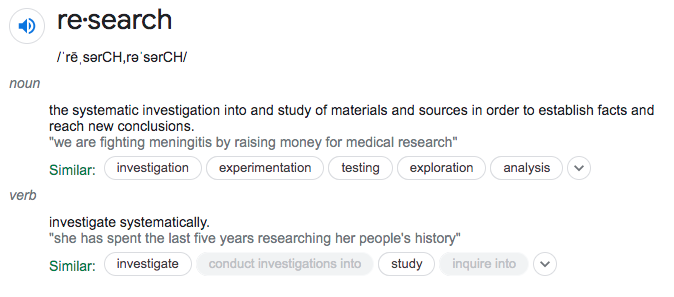
\includegraphics{images/img3.png}
\caption{Definisi umum riset}
\end{figure}
\end{frame}

\hypertarget{alat-metode-dan-pendekatan}{%
\section{Alat, Metode dan Pendekatan}\label{alat-metode-dan-pendekatan}}

\hypertarget{alat}{%
\subsection{Alat}\label{alat}}

\begin{frame}{Google analytics}
\protect\hypertarget{google-analytics}{}
\begin{figure}
\centering
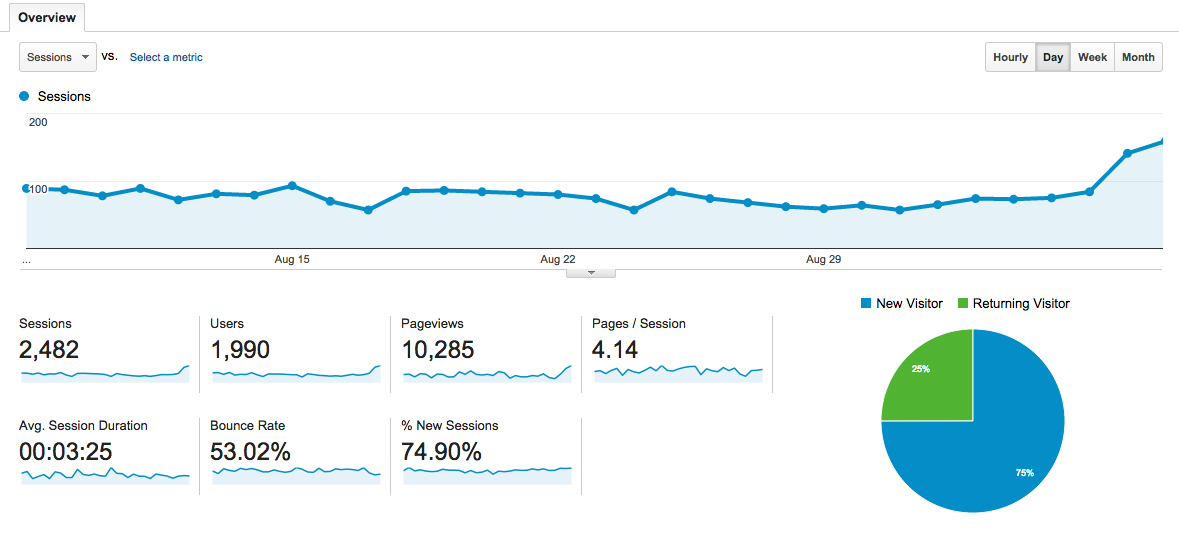
\includegraphics{images/img2.png}
\caption{Google analytics}
\end{figure}
\end{frame}

\begin{frame}{Tebleu}
\protect\hypertarget{tebleu}{}
\begin{figure}
\centering
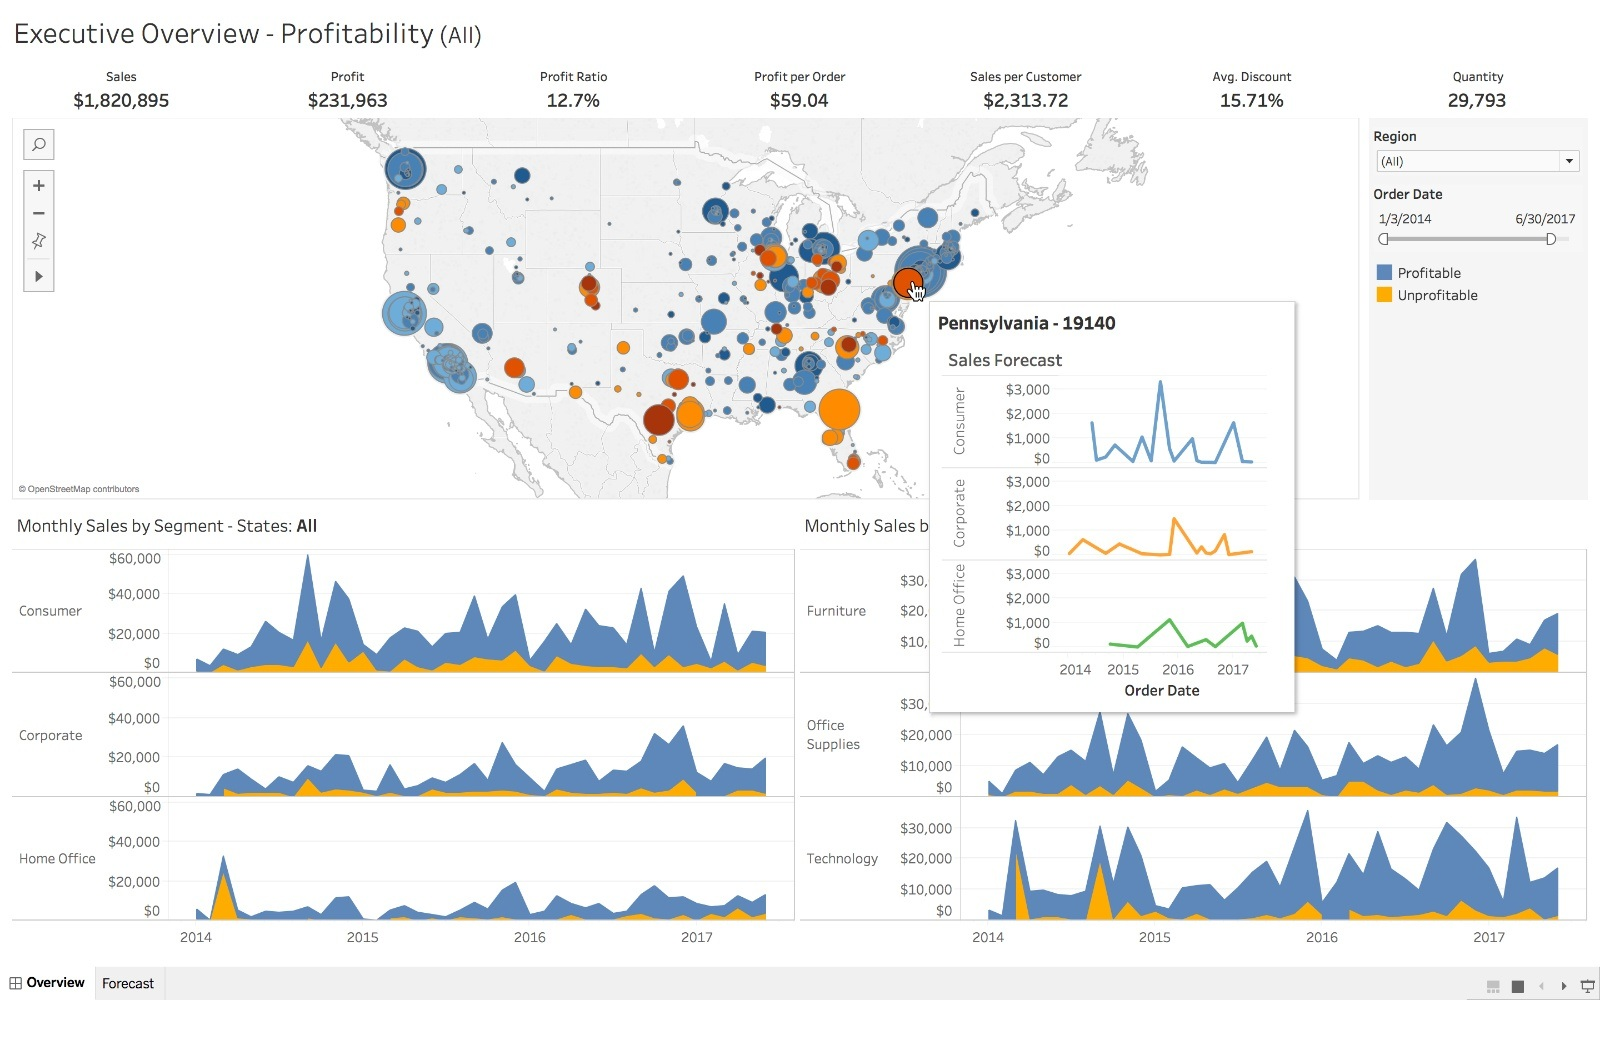
\includegraphics{images/img4.jpeg}
\caption{Tebleu Dashboard}
\end{figure}
\end{frame}

\begin{frame}{Bahasa Pemerograman}
\protect\hypertarget{bahasa-pemerograman}{}
\begin{figure}
\centering
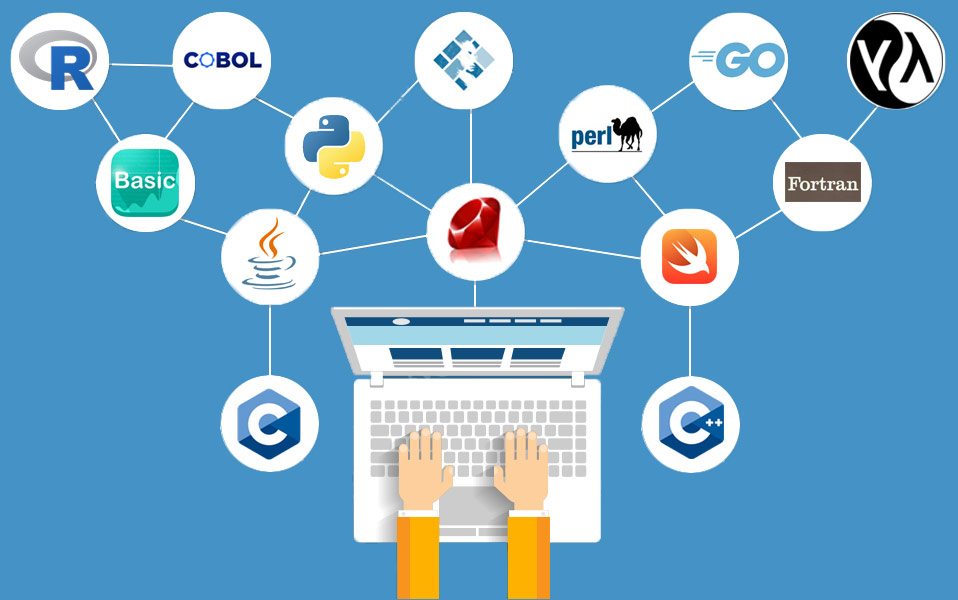
\includegraphics{images/img5.jpeg}
\caption{Berbagai bahasa pemerograman}
\end{figure}
\end{frame}

\begin{frame}{Belajarnya mulai darimana?}
\protect\hypertarget{belajarnya-mulai-darimana}{}
\begin{figure}
\centering
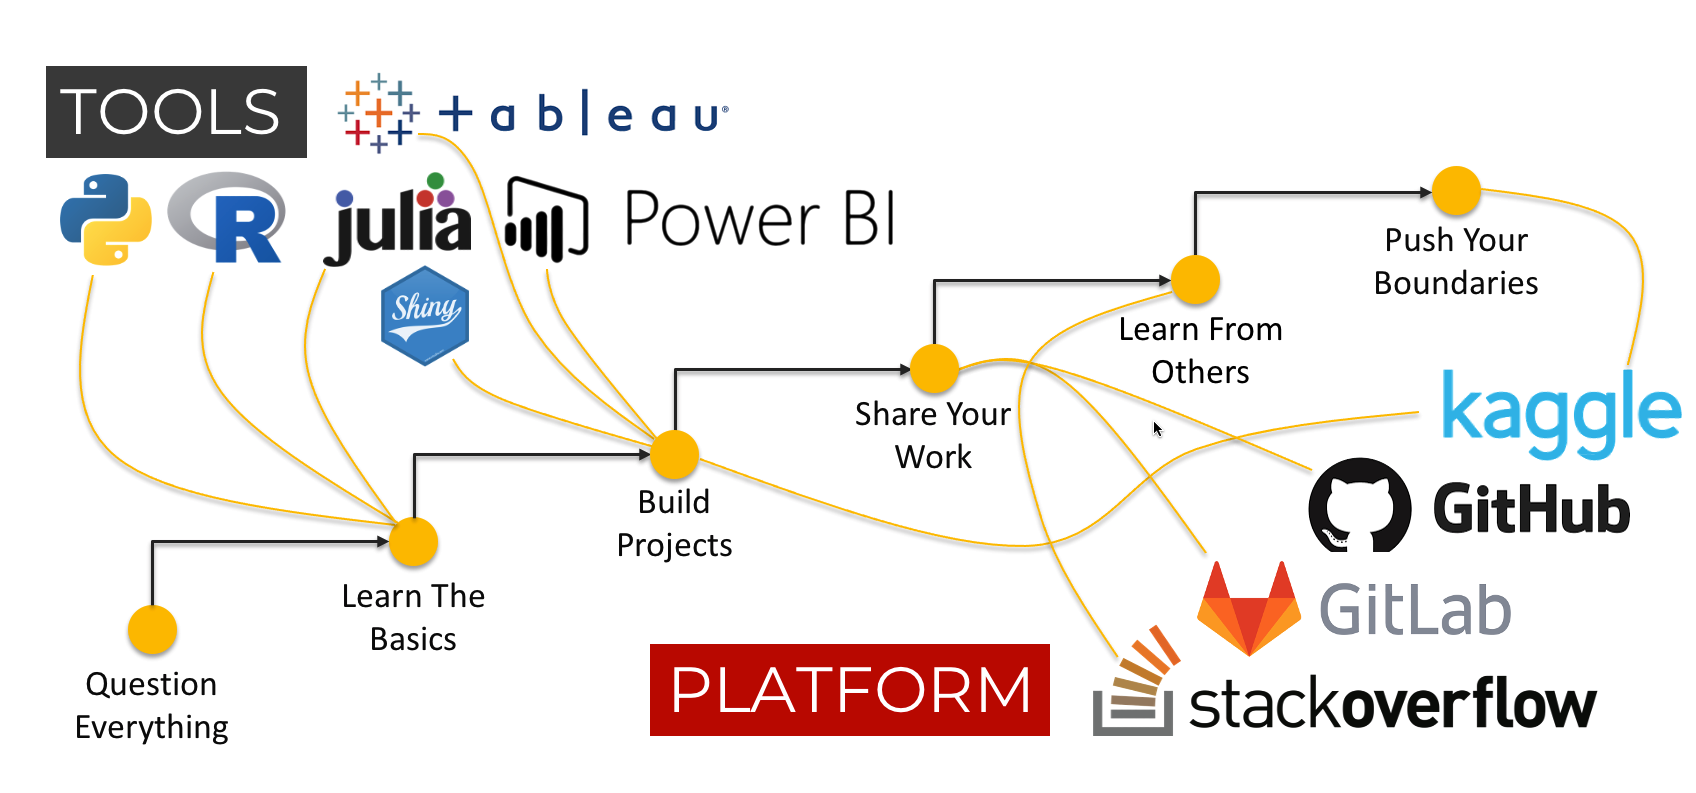
\includegraphics{images/img10.png}
\caption{Alat-alat yang umum digunakan untuk pengoalahan data}
\end{figure}
\end{frame}

\hypertarget{metode}{%
\subsection{Metode}\label{metode}}

\begin{frame}{Metode}
\begin{columns}[T]
\begin{column}{0.5\textwidth}
Secara umum, metode yang biasa digunakan untuk mengolah berbagai data
digital baik yang terstruktur dan tidak terstruktur dapat dibagi menjadi
3, yaitu:

\begin{enumerate}
\tightlist
\item
  Klasifikasi
\item
  Klastering
\item
  Prediksi
\end{enumerate}
\end{column}

\begin{column}{0.5\textwidth}
\begin{figure}
\centering
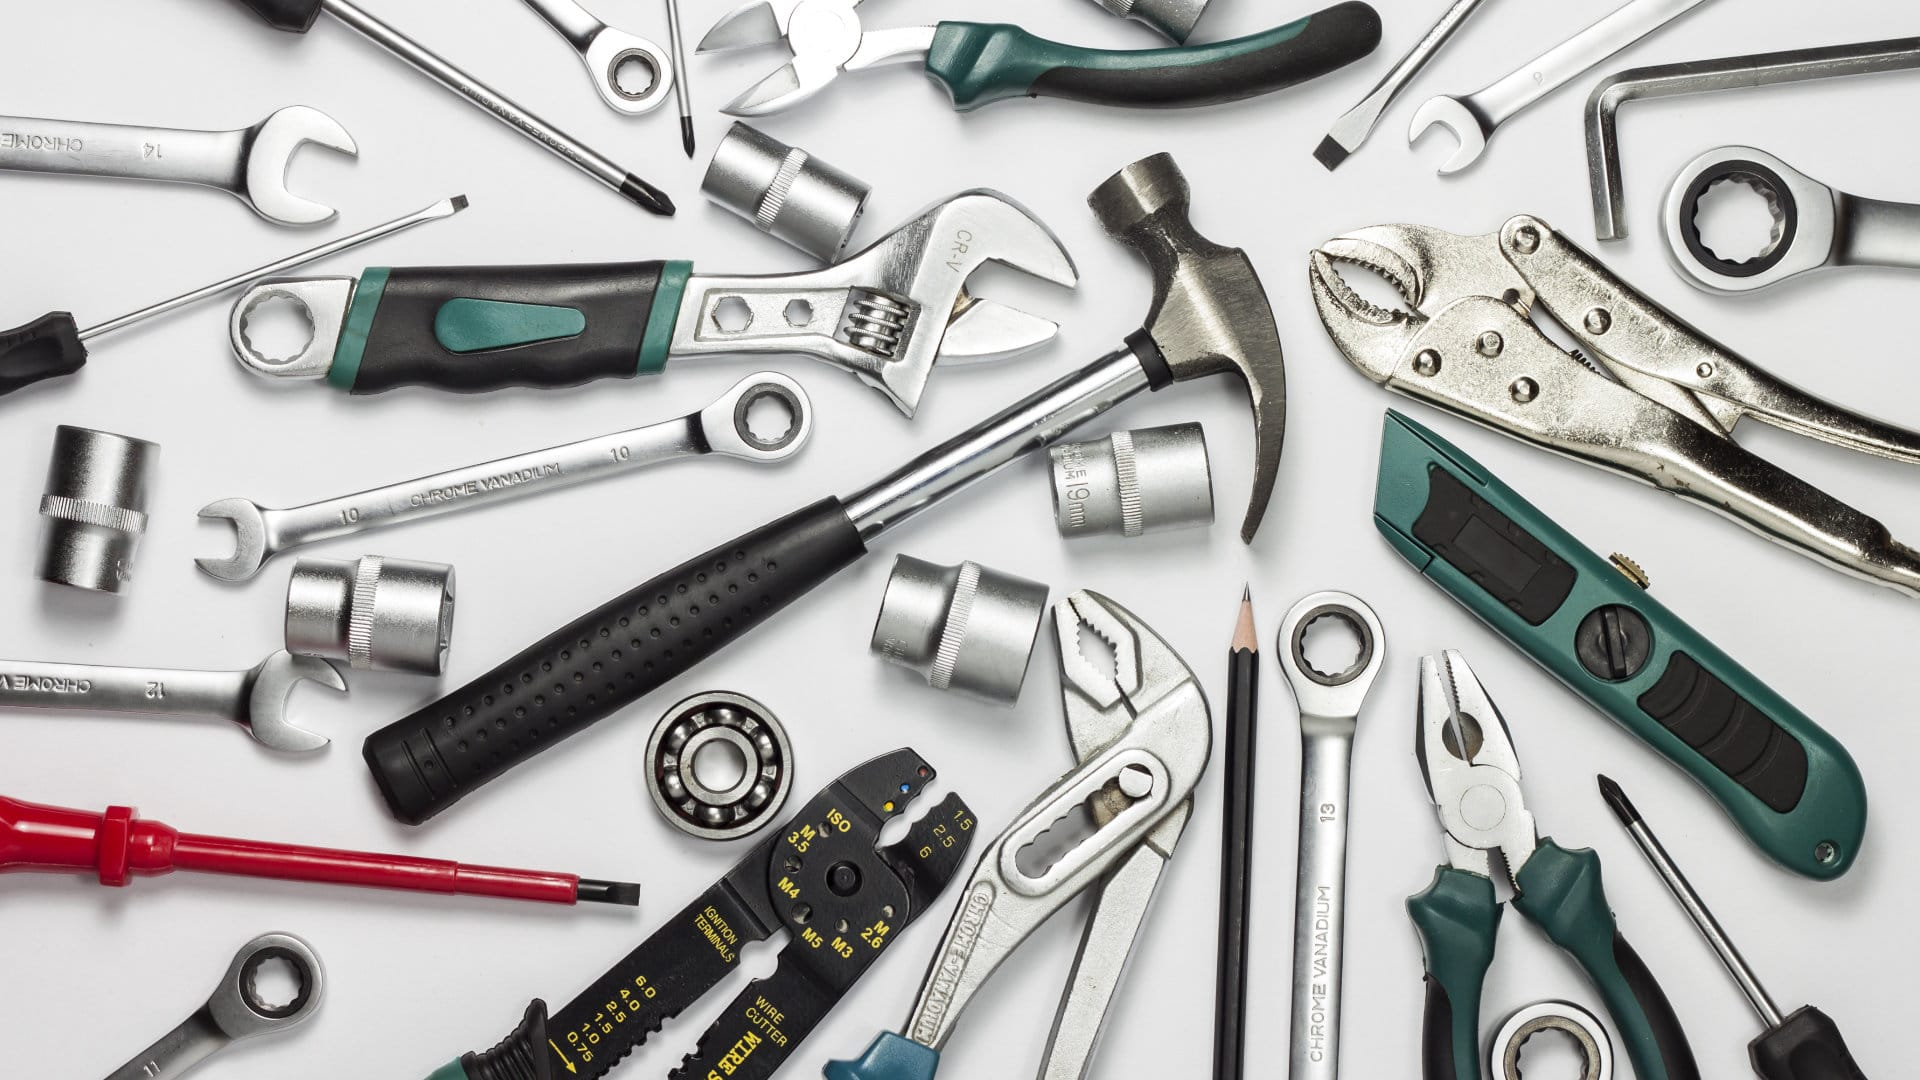
\includegraphics{images/img6.jpeg}
\caption{It just a tools set}
\end{figure}
\end{column}
\end{columns}
\end{frame}

\begin{frame}{Klasifikasi}
\protect\hypertarget{klasifikasi}{}
\begin{columns}[T]
\begin{column}{0.5\textwidth}
Klasifikasi merupakan sebuah proses untuk membuat pengelompokkan
berdasarkan karakteristik yang dimiliki oleh data menjadi
kelompok-kelompok spesifik yang sudah diketahui.

Misalnya, pengelompokkan data siswa berdasarkan gender. Gender yang
mungkin ada sudah diketahui, yaitu Laki-laki dan perempuan.
\end{column}

\begin{column}{0.5\textwidth}
\begin{figure}
\centering
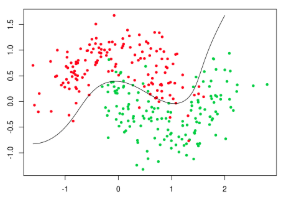
\includegraphics{images/img7.png}
\caption{Hasil klasifikasi sebuah data}
\end{figure}
\end{column}
\end{columns}
\end{frame}

\begin{frame}{Klastering}
\protect\hypertarget{klastering}{}
\begin{columns}[T]
\begin{column}{0.5\textwidth}
Klastering merupakan sebuah proses untuk membuat pengelompokkan
berdasarkan karakteristik yang dimiliki oleh data menjadi
kelompok-kelompok spesifik yang belum diketahui.

Misalnya, pengelompokkan topik pembicaraan warganet di Twitter, dimana
tidak ada informasi yang memberitahu dengan pasti ada berapa topik, dan
topik tentang apa saja.
\end{column}

\begin{column}{0.5\textwidth}
\begin{figure}
\centering
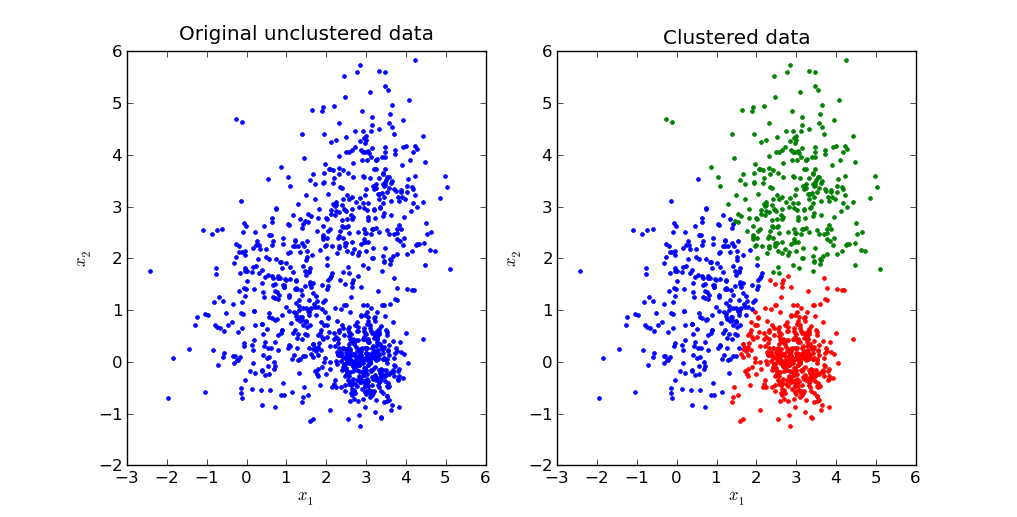
\includegraphics{images/img8.jpeg}
\caption{Ilustrasi klastering}
\end{figure}
\end{column}
\end{columns}
\end{frame}

\begin{frame}{Prediksi}
\protect\hypertarget{prediksi}{}
\begin{figure}
\centering
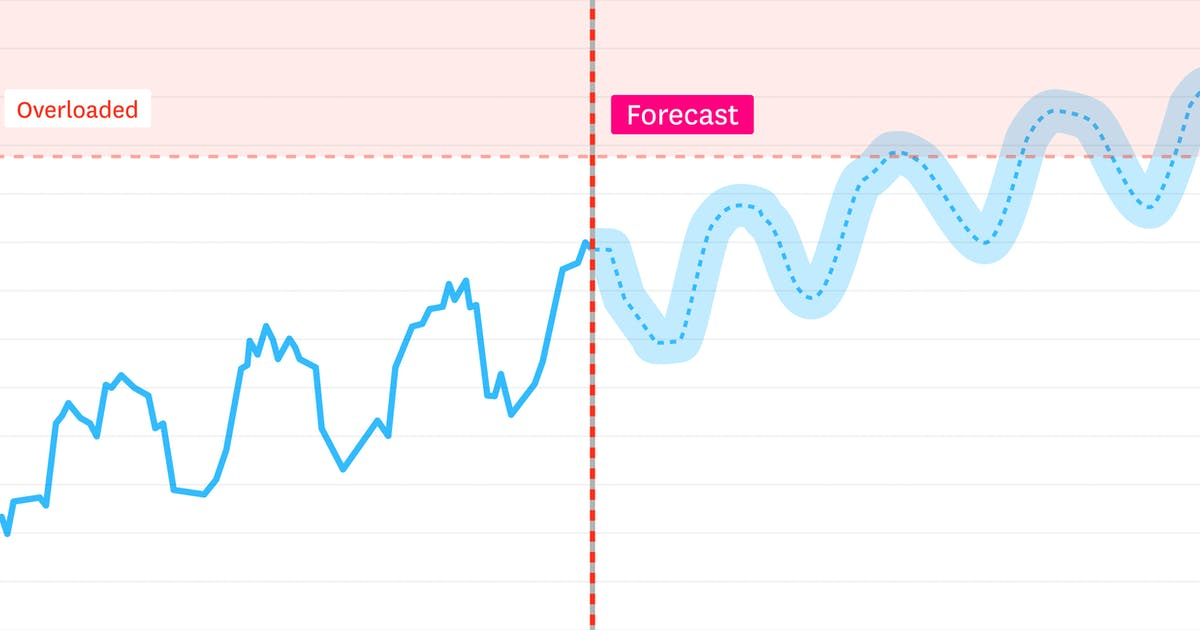
\includegraphics{images/img9.jpeg}
\caption{Ilustrasi prediksi}
\end{figure}
\end{frame}

\hypertarget{analitik-digital}{%
\section{Analitik Digital}\label{analitik-digital}}

\hypertarget{metode-hibrida}{%
\subsection{Metode Hibrida}\label{metode-hibrida}}

\begin{frame}{Metode Hibrida}
Sebuah metode yang menggabungkan antara teknik-tekni data/text mining
dengan metode-metode lain yang sudah lebih dulu stabil sebagai sebuah
cara mengungkap informasi dari dalam sebuah data.
\end{frame}

\begin{frame}{Contoh Kasus}
\protect\hypertarget{contoh-kasus}{}
\begin{itemize}
\item
  Kita ingin mengetahui ada berapa kelompok, dan kelompok apa saja yang
  terlibat dalam sebuah wacana atau tagar yang berkembang di media
  Twitter.
\item
  Karena kita ingin mengetahui kelompok namun belum mengetahui jumlah
  atau jenis pastinya, kita bisa menggunakan metode-metode klastering.
\item
  Metode klastering akan menghasilkan sejumlah kelompok, namun kita
  belum tahu itu kelompok apa saja
\item
  Untuk mengetahui kelompok-kelompok yang ada terkait dengan apa saja,
  langkah logis yang bisa digunakan adalah dengan mengetahui apa yang
  mereka katakan.
\item
  Untuk mengetahui yang mereka katakan, kita perlu melakukan kajian
  terhadap teks yang meraka (per kelompok) posting.
\item
  Langkah paling sederhana untuk mengetahui apa yang tiap kelompok
  katakan adalah dengan mengetahui buzzword (jumlah masing-masing kata
  digunakan)
\item
  Apakah ini sudah cukup? sepertinya belum!
\end{itemize}
\end{frame}

\begin{frame}{Mengetahui konteks kata}
\protect\hypertarget{mengetahui-konteks-kata}{}
\begin{itemize}
\item
  Untuk mengetahui atau bahkan mendefinisikan sesuatu (kelompok)
  berdasarkan yang mereka tulis, kita juga perlu tahu konteks dari tiap
  kata yang dipilih.
\item
  Studi wacana sepertinya cocok dengan karakteristik permasalahan dan
  tujuan analisis yang ingin dicapai
\item
  Ada sebuah metode yang disebut CADS (Corpus assited discourse Studies)
\end{itemize}
\end{frame}

\begin{frame}{Term Network}
\protect\hypertarget{term-network}{}
\begin{columns}[T]
\begin{column}{0.5\textwidth}
Network term, merupakan salah satu bentuk dasar dari jejaring semantik.
Tujuan utamanya adalah untuk mengetahui kata sebelum dan setelahnya.

Dengan pengetahuan kata sebelum dan setelah dan di visualisasi sebagai
network, memungkinkan observer membaca secara keseluruhan konteks dari
kata dan menentukan fokus dengan lebih cepat.
\end{column}

\begin{column}{0.5\textwidth}
\begin{figure}
\centering
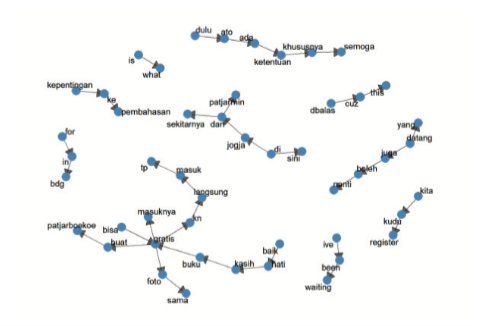
\includegraphics{images/img11.png}
\caption{Jejaring term/kata}
\end{figure}
\end{column}
\end{columns}
\end{frame}

\hypertarget{penutup}{%
\section{Penutup}\label{penutup}}

\begin{frame}{Penutup}
\begin{itemize}
\tightlist
\item
  Setiap penelitian memiliki karakteristik utama yaitu, sistematis dan
  logis
\item
  Metode perlu menyesuaikan tujuan dan data yang akan diolah
\item
  Untuk menggunakan metode campuran, gabungan, atau hibrida, perlu
  penguasaan ilmu yang multidisiplin
\item
  Kolaborasi sepertinya telah menjadi kebutuhan, termasuk dalam
  melakukan penelitian
\end{itemize}
\end{frame}


\section[]{}
\frame{\small \frametitle{Table of Contents}
\tableofcontents}
\end{document}
